%\begin{frame}
%  \vfill
%  \centering
%  %\begin{beamercolorbox}[sep=8pt,center,shadow=true,rounded=true]{block}
%  \begin{sticky}
%    \usebeamerfont{title}
%    {\normalfont\Large MultiParty Session Types} \par%
%  \end{sticky}
%  %\end{beamercolorbox}
%  \vfill
%\end{frame}

\begin{frame}
  \vfill
  \centering
  %\begin{beamercolorbox}[sep=8pt,center,shadow=true,rounded=true]{block}
  \begin{sticky}
    \usebeamerfont{title}
    {\normalfont Background}

    {\normalfont\Large Hylomorphisms}
    \par%
  \end{sticky}
  %\end{beamercolorbox}
  \vfill
\end{frame}

\begin{frame}[fragile]
  \frametitle{Fold over Lists}

  One way to guarantee \embf{recursive functions} are \embf{well-defined} is
  via \embf{Recursion Schemes}.

  \vspace{.6cm}

  \begin{minted}{Haskell}
foldr :: (a -> b -> b) -> b -> [a] -> b
foldr g b [] = b
foldr g b (x : xs) = g x (foldr g b xs)
  \end{minted}

  \vspace{.6cm}

  There are many different kinds of Recursion Schemes (e.g. Folds,
  Paramorphisms, Unfolds, Apomorphisms, \ldots)
\end{frame}

\begin{frame}[fragile]
  \frametitle{Folds as Initial Algebras}
  \centering

  \begin{columns}
    \begin{column}{.52\textwidth}
      \begin{minted}[escapeinside=??]{Haskell}
data Fix f = In { inOp :: f (Fix f) }

fold :: Functor f =>
          (f x -> x) -> 
          Fix f -> 
          x
fold a = f
    where f (In?\tikzmark{algIni1}? x) = (a?\tikzmark{alg1}? . fmap f) x
      \end{minted}
    \end{column}
    \begin{column}{.37\textwidth}
      \begin{tikzcd}
        \mhask{f (Fix f)} \arrow[r, dotted] \arrow[d, swap, "\mhask{In}"] 
        & \mhask{f x} \arrow[d, "\mhask{a}"] 
        \\
        \mhask{Fix f}\tikzmark{algIni2} \arrow[r, dotted] 
        & \mhask{x}\tikzmark{alg2}
\end{tikzcd}
    \end{column}
  \end{columns}

  \begin{onlyenv}<2>
  \begin{tikzpicture}[overlay,remember picture,shift=(current page.south west)]
    \node[rectangle, rounded corners, fill=yellow!80!black] at (11,6.5) 
    {\begin{tabular}{@{}c@{}}
      Least Fixed-Point  \\
      $\mhask{Fix f} \cong \mhask{f (Fix f)}$
    \end{tabular}}; 
  \end{tikzpicture}
  \end{onlyenv}
  \begin{onlyenv}<3>
  \begin{tikzpicture}[overlay,remember picture,shift=(current page.south west)]
    \node[rectangle, rounded corners, fill=yellow!80!black] at (10,1) (a) 
      {\haskell{f}-algebra}; 

    \draw[overlay, yellow!80!black, arrows=->, line width=.5mm]
      (a.west) -- (pic cs:alg1);
    \draw[overlay, yellow!90!black, arrows=->, line width=.5mm]
      (a.east) -- ($(pic cs:alg2) + (-.1, -.2)$);
  \end{tikzpicture}
  \end{onlyenv}
  \begin{onlyenv}<4>
  \begin{tikzpicture}[overlay,remember picture,shift=(current page.south west)]
    \node[rectangle, rounded corners, fill=yellow!80!black] at (7,1) (a) 
      {initial \haskell{f}-algebra}; 

    \draw[overlay, yellow!80!black, arrows=->, line width=.5mm]
      (a) -- (pic cs:algIni1);
    \draw[overlay, yellow!90!black, arrows=->, line width=.5mm]
      (a) -- ($(pic cs:algIni2) + (-.8, -.2)$);
  \end{tikzpicture}
  \end{onlyenv}
\end{frame}


\begin{frame}[fragile]
  \frametitle{Hylomorphisms: Divide-and-conquer Computations}
  \centering
  
  \begin{columns}
    \begin{column}{.52\textwidth}
      \begin{minted}[escapeinside=??]{Haskell}
hylo :: Functor f =>
          (f b -> b) -> 
          (a -> f a) -> 
          a -> b
hylo a c = a ?\tikzmark{halg1}? . fmap (hylo a c) . c ?\tikzmark{hcoalg1}?
      \end{minted}
    \end{column}
    \begin{column}{.37\textwidth}
      \begin{tikzcd}
        \mhask{f a} \arrow[r, dotted] 
        & \mhask{f b} \arrow[d, "\mhask{a}"] 
        \\
        \mhask{a}\tikzmark{hcoalg2} \arrow[u, "\mhask{c}"] \arrow[r, dotted] 
        & \mhask{b}\tikzmark{halg2}
\end{tikzcd}
    \end{column}
  \end{columns}

  \begin{onlyenv}<3>
  \begin{tikzpicture}[overlay,remember picture]
    \node[rectangle, rounded corners, fill=yellow!80!black] at (2,-1) (ha) 
      {\begin{tabular}{@{}c@{}}
        \haskell{f}-algebra \\
        ``conquer''
      \end{tabular}}; 

    \draw[overlay, yellow!90!black, arrows=->, line width=.5mm]
      (ha) -- (pic cs:halg1);
    \draw[overlay, yellow!90!black, arrows=->, line width=.5mm]
      (ha) -- ($(pic cs:halg2) + (-.1, -.2)$);
  \end{tikzpicture}
  \end{onlyenv}

  \begin{onlyenv}<2>
  \begin{tikzpicture}[overlay,remember picture]
    \node[rectangle, rounded corners, fill=yellow!80!black] at (9,-1.5) (hc) 
      {\begin{tabular}{@{}c@{}}
        \haskell{f}-coalgebra \\
        ``divide''
      \end{tabular}}; 

    \draw[overlay, yellow!90!black, arrows=->, line width=.5mm]
      (hc) -- (pic cs:hcoalg1);
    \draw[overlay, yellow!90!black, arrows=->, line width=.5mm]
      (hc) -- ($(pic cs:hcoalg2) + (-.1, -.2)$);
  \end{tikzpicture}
  \end{onlyenv}
\end{frame}

\begin{frame}[fragile]
  \frametitle{Folds as Hylomorphisms}
  \centering
  
  \begin{columns}
    \begin{column}{.52\textwidth}
      \begin{minted}[escapeinside=??]{Haskell}
data Fix f = In { inOp :: f (Fix f) }

fold :: Functor f =>
          (f x -> x) -> 
          Fix f -> 
          x
fold a = a?\tikzmark{fhalg1}? . fmap (fold a) . inOp?\tikzmark{fhcoalg1}?
      \end{minted}
    \end{column}
    \begin{column}{.37\textwidth}
      \begin{tikzcd}
        \tikzmark{fhcoalg2}\mhask{f (Fix f)} \arrow[r, dotted] 
        & \mhask{f x} \arrow[d, "\mhask{a}"] 
        \\
        \mhask{Fix f} \arrow[u, "\mhask{inOp}"] \arrow[r, dotted] 
        & \mhask{x}\tikzmark{fhalg2}
\end{tikzcd}
    \end{column}
  \end{columns}

  \begin{tikzpicture}[overlay,remember picture]
    \node[rectangle, rounded corners, fill=yellow!80!black] at (2,-1) (fha) 
      {\haskell{f}-algebra}; 

    \draw[overlay, yellow!90!black, arrows=->, line width=.5mm]
      (fha) -- ($(pic cs:fhalg1) + (.2, 0)$);
    \draw[overlay, yellow!90!black, arrows=->, line width=.5mm]
      (fha) -- ($(pic cs:fhalg2) + (-.1, -.2)$);
  \end{tikzpicture}

  \begin{tikzpicture}[overlay,remember picture]
    \node[rectangle, rounded corners, fill=yellow!80!black] at (9,4) (fhc) 
      {\haskell{f}-coalgebra}; 

    \draw[overlay, yellow!90!black, arrows=->, line width=.5mm]
      (fhc) -- ($(pic cs:fhcoalg1) + (-.2, .3)$);
    \draw[overlay, yellow!90!black, arrows=->, line width=.5mm]
      (fhc) -- ($(pic cs:fhcoalg2) + (.7, .4)$);
  \end{tikzpicture}
\end{frame}

\begin{frame}[fragile]
  \frametitle{Example: Nonstructural Recursion}
  \centering

  \begin{columns}
    \begin{column}{.5\textwidth}
      \begin{minted}[escapeinside=??, fontsize=\scriptsize]{Haskell}
data TreeF a b = Leaf |  Node b a b

split [] = Leaf?\tikzmark{qscoalg1}?
split (h : t) = Node l h r
  where
    (l, r) = partition (\x -> x < h) t

merge Leaf = \acc -> acc
merge (Node l x r) = \acc -> l (x : r acc)?\tikzmark{qsalg1}?
      \end{minted}
    \end{column}
    \begin{column}{.47\textwidth}\scriptsize
      \begin{tikzcd}
        \tikzmark{qscoalg2}\mhask{TreeF Int [Int]} \arrow[r, dotted, "\mhask{fmap qsort}"] 
        & \mhask{TreeF Int ([Int] -> [Int])} \arrow[d, "\mhask{merge}"] 
        \\
        \mhask{[Int]} \arrow[u, "\mhask{split}"] \arrow[r, dotted, "\mhask{qsort}"] 
        & \mhask{[Int] -> [Int]}\tikzmark{qsalg2}
\end{tikzcd}
    \end{column}
  \end{columns}

  \begin{onlyenv}<2>
  \begin{tikzpicture}[overlay,remember picture,shift=(current page.south west)]
    \node[rectangle, rounded corners, fill=yellow!80!black] at (12,2) (qsa) 
      {\haskell{TreeF Int}-algebra}; 

    \draw[overlay, yellow!90!black, arrows=->, line width=.5mm]
      (qsa) -- ($(pic cs:qsalg1) + (.2, 0)$);
    \draw[overlay, yellow!90!black, arrows=->, line width=.5mm]
      (qsa) -- ($(pic cs:qsalg2) + (-1, -.2)$);
  \end{tikzpicture}

  \begin{tikzpicture}[overlay,remember picture,shift=(current page.south west)]
    \node[rectangle, rounded corners, fill=yellow!80!black] at (10,7) (qsc) 
      {\haskell{TreeF Int}-coalgebra}; 

    \draw[overlay, yellow!90!black, arrows=->, line width=.5mm]
      (qsc) -- ($(pic cs:qscoalg1) + (.2, .3)$);
    \draw[overlay, yellow!90!black, arrows=->, line width=.5mm]
      (qsc) -- ($(pic cs:qscoalg2) + (1, .4)$);
  \end{tikzpicture}
  \end{onlyenv}
\end{frame}

% \begin{frame}[fragile]
%   \frametitle{Adjoint Folds}
%   Given an adjunction:
% 
%   \begin{center}\LARGE
%   \begin{tikzcd}
%     \mathcal{D} \arrow[r, swap, "\mathsf{R}"{name=G}, bend right=25] &
%     \mathcal{C} \arrow[l, swap, "\mathsf{L}"{name=F}, bend right=25]
%     \arrow[phantom, from=F, to=G, "\dashv" rotate=-90]
%   \end{tikzcd}
%   \end{center}
% 
%  \begin{itemize}
%    \item There is a correspondence of arrows 
%      $\lfloor\cdot\rfloor : \mathsf{Hom}_{\mathcal{D}}(L\, A,B) \cong 
%      \mathsf{Hom}_{\mathcal{C}}(A,R\, B) : \lceil\cdot\rceil$.
%    \item An initial algebra on the right corresponds to an universal property
%      on the left:
%      {\large
%      \[
%        \mathsf{Hom}_{\mathcal{D}}(L\, \mu F, B) \cong \mathsf{Hom}_{\mathcal{C}}(\mu F,R\, B)
%      \]}\blfootnote{$\mu$ analogous to Haskell's \haskell{Fix}}\blfootnote{$F$
%      is an endofunctor in $\mathcal{C}$}\blfootnote{$L$, $R$ are functors
%      between $\mathcal{C}$ \& $\mathcal{D}$; the \emph{left} and \emph{right}
%      adjoints.}
%  \end{itemize}
% \end{frame}
%  %\arrow[phantom, from=F, to=G, "\dashv" rotate=-90, no line]

% NOTES:
% - Every complex recursion scheme is an hylomorphism via its associated
%   adjunction/conjugate pair 

% - (e.g) folds with parameters (accumulators) use the curry/uncurry adjunction 

% - a recursion scheme from comonads (RSFCs, Uustalu, Vene, Pardo, 2001) is an
%   conjugate hylomorphism via the coEilemberg-Moore category for the cofree
%   comonad.
\begin{frame}[fragile]
  \frametitle{Conjugate Hylomorphisms}
  \centering
  {\Large\emph{Every recursion scheme is a conjugate hylomorphism}}%
  \blfootnote{\tiny{}R. Hinze, N. Wu, J. Gibbons: \textbf{Conjugate
  Hylomorphisms - Or: The Mother of All Structured Recursion Schemes}. POPL
  2015.}

  \vspace{.4cm}

  \begin{sticky}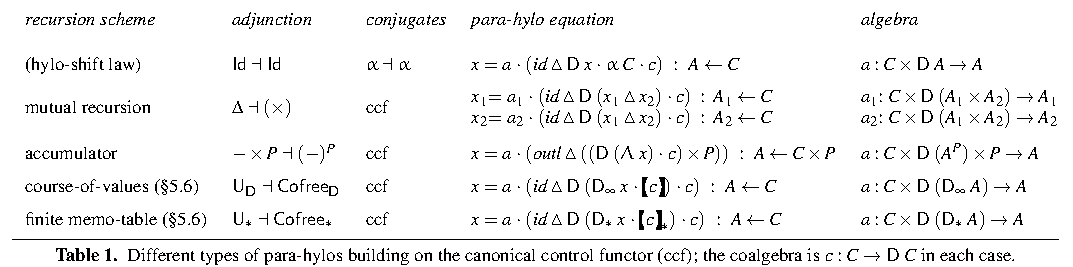
\includegraphics[width=\textwidth]{figures/types-of-parahylos-crop.pdf}\end{sticky}
\end{frame}

\begin{frame}
  \frametitle{Why Mechanising Hylomorphisms in Coq?}

  \begin{itemize}
    \item Structured Recursion Schemes have been used in Haskell to structure
      functional programs, but they do not ensure termination/productivity
    \item On the other hand, Coq does not capture all recursive definitions
    \item The benefits of formalising hylos in Coq is three fold:
      \begin{itemize}
        \item Giving the Coq programmer a \embf{library} where for most
          recursion schemes they do not have to prove termination properties
        \item \embf{Extracting code} into ML/Haskell to provide termination
          guarantees even in languages with non-termination
        \item Using the laws of hylomorphisms as tactics for \embf{program
          calculation} and \embf{optimisation}
      \end{itemize}
  \end{itemize}
\end{frame}

\begin{frame}
  \frametitle{Challenges}
  \begin{enumerate}
    \item Avoiding axioms: functional extensionality, heterogeneous equality,
      \ldots.
    \item Extracting ``clean'' code: close to what a programmer would have
      written directly in OCaml.
    \item Fixed-points of functors, non-termination, etc.
  \end{enumerate}

  \vspace{.5cm}
  
  \uncover<2->{%
    Our solutions (the remainder of this talk):
    \begin{enumerate}
      \item<2-> Machinery for building setoids, use of decidable predicates, \ldots
      \item<3-> Avoiding type families and indexed types.
      \item<4-> \embf{Containers} \& \embf{recursive coalgebras}
    \end{enumerate}
   }
\end{frame}


\begin{frame}
  \frametitle{Roadmap}
  \centering
  \LARGE

    \begin{sticky}%
      \vspace{-1.5em}
      \begin{tabular}{@{}rl}
        {\textbf{\color{gray}Part I:}} & Extractable Containers in Coq \\
        {\textbf{\color{gray}Part II:}} & Recursive Coalgebras \& Coq Hylomorphisms \\
        {\textbf{\color{gray}Part III:}} & Code Extraction \& Examples 
      \end{tabular}
    \end{sticky}
\end{frame}
% 
% \begin{frame}
%   \frametitle{Why Mechanising Hylomorphisms in Coq?}
% 
%   \begin{itemize}
%   \end{itemize}
% \end{frame}
% 
\begin{frame}
  \vfill
  \centering
  %\begin{beamercolorbox}[sep=8pt,center,shadow=true,rounded=true]{block}
  \begin{sticky}
    \usebeamerfont{title}
    {\normalfont Part I}

    {\normalfont\Large Extractable Containers in Coq}
    \par%
  \end{sticky}
  %\end{beamercolorbox}
  \vfill
\end{frame}

\begin{frame}
  \vfill
  \centering
  %\begin{beamercolorbox}[sep=8pt,center,shadow=true,rounded=true]{block}
  \begin{sticky}
    \usebeamerfont{title}
    {\normalfont Part II}

    {\normalfont\Large Recursive Coalgebras \& Coq Hylomorphisms}
    \par%
  \end{sticky}
  %\end{beamercolorbox}
  \vfill
\end{frame}

\begin{frame}
  \vfill
  \centering
  %\begin{beamercolorbox}[sep=8pt,center,shadow=true,rounded=true]{block}
  \begin{sticky}
    \usebeamerfont{title}
    {\normalfont Part III}

    {\normalfont\Large Code Extraction \& Examples}
    \par%
  \end{sticky}
  %\end{beamercolorbox}
  \vfill
\end{frame}


\begin{frame}
  \vfill
  \centering
  %\begin{beamercolorbox}[sep=8pt,center,shadow=true,rounded=true]{block}
  \begin{sticky}
    \usebeamerfont{title}
    {\normalfont Wrap-up}

    {\normalfont\Large \phantom{wrap-up}}
    \par%
  \end{sticky}
  %\end{beamercolorbox}
  \vfill
\end{frame}

\begin{frame}
  
\end{frame}
